\section{\LaTeX HowTo for this Template}
\label{sec:2}


\cappar In this Chapter I explain some \LaTeX tips and tricks for this template. In case you don't agree with my proposals please adapt the template to your needs and individual preferences.

\vspace{.6cm}
\secttoc
\vspace{.6cm}

\subsection{Sections}
As we are not using a book-style there is no \texttt{\textbackslash chapter\{\}} option. Thus the top-level titles are generated by means of \texttt{\textbackslash section\{\}}. Second level headers are then generated with  \texttt{\textbackslash subsection\{\}}. Note that we only sections and subsections go into the table of content.

\subsection{Fancy Chapter Beginning}
Each chapter starts with a short text with up to ten lines which describes briefly what is in the chapter. In order to generate a large starting letter type \texttt{\textbackslash cappar} in front of the introductory text. The local table of context is generated by means of the following commands \newline \newline \texttt{\textbackslash vspace{.6cm} \\ \textbackslash secttoc \\ \textbackslash vspace{.6cm}} \newline \newline Note that only subsections go into the local table of content per chapter.

\subsection{Pdf-Output settings}
You configure certain pdf-output parameters (e.g. title of the generated file) in \texttt{formatAndDefs.tex} around line $65$.

\subsection{Figures}
Figures are generated as usual with the \texttt{\textbackslash begin\{figure\}} command.

\begin{figure}
	\centering
	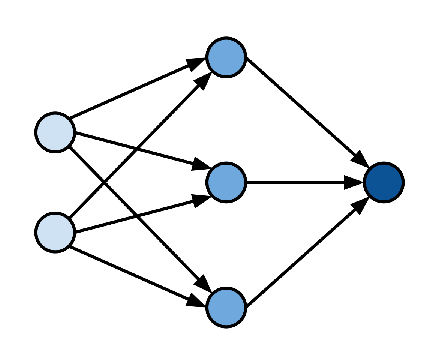
\includegraphics[width=.45\textwidth]{nn.pdf}
	\caption{Neural network with one hidden layer}
	\label{fig:ex}
\end{figure}

\subsection{Algorithms}
Algorithms can be generated by means of the algorithmic package. An exemplary output looks like \autoref{alg:ex}. We refer to the source code of this document or to the algorithmic package documentation for detailed information.


\begin{algorithm}\caption{Automatic Thresholding Algorithm}\label{alg:ex}
	\begin{algorithmic}
	\STATE Init: Initial guess $T$, Tolerance $\epsilon$
	\STATE $dt := 2\epsilon$
	\WHILE {$(dt > \epsilon)$}
		\STATE $G_1 := \begin{Bmatrix} I_{i,j}: I_{i,j} > T \end{Bmatrix}$
		\STATE $G_2 := \begin{Bmatrix} I_{i,j}: I_{i,j} \leq T \end{Bmatrix}$
		\STATE $m_1 :=$ Average value of $G_1$
		\STATE $m_2 :=$ Average value of $G_2$
		\STATE $T' = \frac{(m_1 + m_2)}{2}$
		\STATE $dt = \lvert T - T' \rvert$
		\STATE $T = T'$
	\ENDWHILE
	\STATE return T
	\end{algorithmic}
\end{algorithm}

\subsection{Tables}
\autoref{tab:ex} shows an example of a table. Adapt the source code of this documents to your needs and check the booktabs package documentation, which is used in the present template.

\begin{table}
	\centering
	\caption{Comparison of the segmentation performance}
	\label{tab:ex}
	\begin{tabular}{l l c c c}
		\toprule

		%\multicolumn{2}{l}{\textbf{Class}  stat. Method} \\
		\textbf{Class} & \textbf{stat. Method} \hspace{0.6cm} & \multicolumn{3}{l}{\textbf{Segmentation accuracy in \% $\pm \text{ 1 } \sigma$}}\\
		\cmidrule{1-5}
		Background &  & correct & $\rightarrow$ DNA strand \\ 
		\cmidrule{3-5}
			 & PostProcessing(SVM) 	& $ 99.545 \pm 0.081 $ & $ 0.455 \pm 0.081 $ \\
			 & USZ-Method			& $ 99.798 \pm 0.039 $ & $ 0.202 \pm 0.039 $ \\
			 & Cancer Research App	& $ 99.973 \pm 0.013 $ & $ 0.027 \pm 0.013 $ \\

		\cmidrule{1-5}
		DNA strand &  & correct & $\rightarrow$ Background \\ 
		\cmidrule{3-5}
			 & PostProcessing(SVM) 	& $ 96.704 \pm 1.288 $ & $ 3.296 \pm 1.288 $ \\
			 & USZ-Method			& $ 84.795 \pm 1.556 $ & $ 15.204 \pm 1.556 $ \\
			 & Cancer Research App	& $ 95.513 \pm 2.03 $ & $ 4.488 \pm 2.03 $ \\

		\bottomrule
	\end{tabular}
\end{table}


\subsection{Listings}
All listing should be stored in the codesamples subfolder and they are included with \texttt{\textbackslash lstinputlisting[caption=..., float=tbph, label=...]{codesamples/listname}}. The current setting is optimized for C++. Adapt the settings to your needs in formatAndDefs.tex around line $30$. In case you need other keywords (e.g. Cuda stuff) add the keywords to the list of "morekeywords in Line $52$ in the formatAndDefs.tex file. \autoref{list:ex} shows a trivial listing example.

\lstinputlisting[caption=\texttt{int main} example listing, float=tbph, label=list:ex] {codesamples/intmain.cpp}

\subsection{AutoRefs}
Instead of \texttt{\textbackslash ref} we use \texttt{\textbackslash autoref} which generate better looking links, e.g. \autoref{fig:ex}, \autoref{alg:ex}, \autoref{tab:ex} or \autoref{list:ex}. The keywords can be change around line $186$ in formatAndDefs.tex.

\subsection{References}
All references are generated as usual with \texttt{\textbackslash cite}. The only difference is that we generate a back-link from the list of references to the place where you cited the reference. For example you see under the references that I cited \cite{wiki} on this page. In addition all references are links.

\subsection{General formating}
Play around with empty pages between the different chapters in order to ensure that all chapters begin on a right page.


